% Describe the test setup to verify that your problems from 1.3 have been solved.
% This can be done in different ways depending on focus of your problems.
% Some problems may purely objective, such as "improve the performance of X compared to Y".
% These are easy to evaluate since you simply need to compare the performance, and perhaps compare against a few more technologies that you have listed in Section 2 (related work).
% In other cases the problems may be very subjective, such as "Create a mobile app that can be used while driving, and which shows the most fuel efficient time to change gear".
% This problem will require a user-study in which several persons drive without the application, you calculate the fuel consumption, then they drive with the application and then you calculate the fuel consumption again.
% Then you collect the objective measurements (fuel consumption comparisons) and the subjective opinions from the users about whether the application was unobtrusive, usable, etc. (typically via a questionnaire).

% Move to above section
The example code used to test is not totaly a real program that would be worked on because it would take to much time making or finding such examples that covers all the different cases that a debugger encounters.
But that said all debuggers have been tested on real code examples as well to see that they work.


Now comparing the debugger is done by manuly debugging example code \cite{debugexample} and looking for diffrences in the result.
The version of \gls{gdb} used is \emph{gdb-11.0} because it is the latest version released on the latest \emph{Ubuntu} version which is \emph{Ubuntu 21.04}.
For the same reason the version of \emph{lldb} used is version $10.1$.


When running the example code on optimization $2$ and with a software breakpoint set in the middle of a function to ensure that both debugger stop on the same machine code location.
The \emph{GDB} debugger gave a wrong answer when debugging the value of a enum named \emph{test\_enum3}, the value that \emph{GDB} can be seen in figure \ref{fig:gdbenum}.
The expected value is \emph{TODO} which is not the same as what \emph{GDB} gave.
Doing the same using the debugger presented in this thesis shows that it also is not the same value as expected, the result can be seen in  figure \ref{fig:mydebuggerenum}.
The printing look a bit diffrent but the result from the debugger presented in this thesis tells the user that the enum \emph{test\_enum3} is a enum of type \emph{TestEnum} where the acatual variant has been optimized out.
While \emph{GDB} also tells that \emph{test\_enum3} is of type \emph{TestEnum} and that it is of the enum variant \emph{ITest} where the value is optimized out.
As can be seen \emph{GDB} gives the wrong answere because it says that \emph{test\_enum3} is the enum variant \emph{TestEnum::ITest} which is wrong.
While the debugger presesneted in this thesis says that the value has been optimized out which is a more correct anwser.
Doing the same using \gls{lldb} give almost the smae result as the debugger presented in this thesis and that result can be seen in figure \ref{fig:lldbenum}.
\gls{lldb} dosnet print that the variant of the enum has been optimized out which makes the reason why it is not printed ambigius.


\begin{figure}[h]
    \centering
    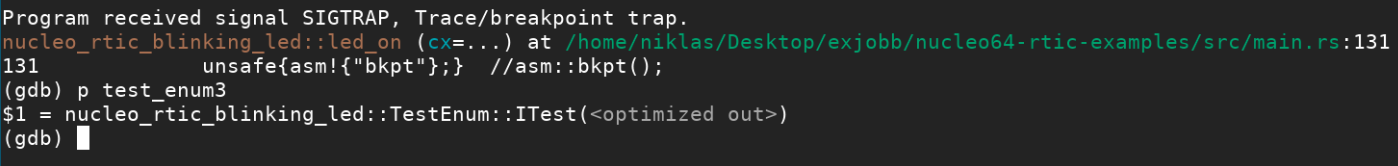
\includegraphics[width=1.0\textwidth]{gdb10.1-opt2-enum-edited.png}
    \label{fig:gdbenum}
\end{figure}


\begin{figure}[h]
    \centering
    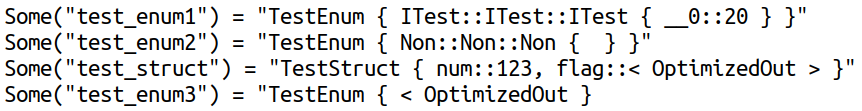
\includegraphics[width=1.0\textwidth]{my-debugger-opt2-enum-edited.png}
    \label{fig:mydebuggerenum}
\end{figure}


\begin{figure}[h]
    \centering
    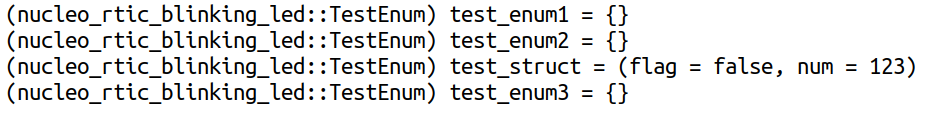
\includegraphics[width=1.0\textwidth]{lldb11.0-opt2-enum-edited.png}
    \label{fig:lldbenum}
\end{figure}


Now when inspecting what is stored in the \emph{DWARF} format is shows that the variant of the enum is optimized out but not the two other values that make up the value stored in the variant.
The fact that the value that indicate with variant is optimized out makes it impossible for any debugger to evalute the value stored in the enum.
This is because the encoding of the bytes is unknown and because the number of bytes to read from the stack is unknown.


Looking back at figure \ref{fig:lldbenum} there are three other enums there where two of them dosen't have a value as well, they are named \emph{test\_enum1} and \emph{test\_enum2}.
Those two enums should have a value but for some reason \gls{lldb} is not able to evaluate them, but looking at figure \ref{fig:mydebuggerenum} shows the values they should have.
Also looking at figure \ref{fig:gdbenum} shows the same result as in figure \ref{fig:mydebuggerenum} thus both \gls{gdb} and the debugger presented in this thesis is able to evaluate the correct value.

Going back again to figure \ref{fig:lldbenum} which shows that the value of the attribute \emph{flag} is equal to \emph{false}, but looking at figure \ref{fig:gdbenum} and \ref{fig:lldbenum} shows that the value of \emph{flag} is equal to \emph{true}.
The correct value when looking at the original source code is that the attribute \emph{flag} should be equal to \emph{true}, thus meaning that the result from \gls{lldb} is incorrect.




\begin{figure}[h]
    \centering
    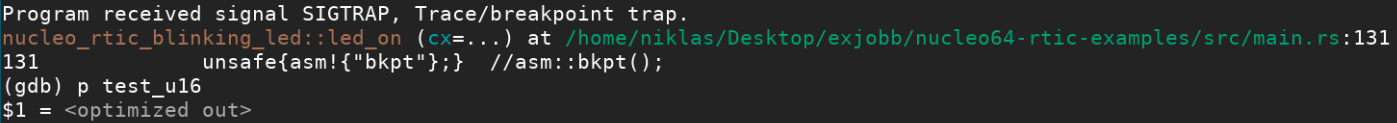
\includegraphics[width=1.0\textwidth]{gdb10.1-opt2-outofrange-edited.png}
    \label{fig:gdboutofrange}
\end{figure}


\begin{figure}[h]
    \centering
    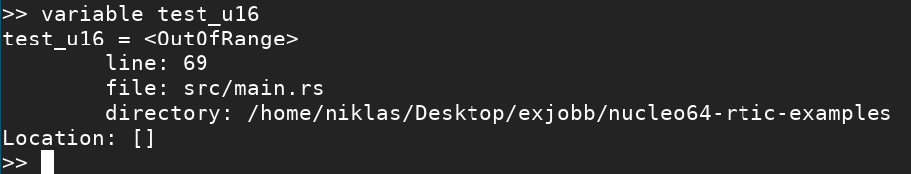
\includegraphics[width=1.0\textwidth]{my-debugger-opt2-outofrange-edited.png}
    \label{fig:mydebuggeroutofrange}
\end{figure}


\begin{figure}[h]
    \centering
    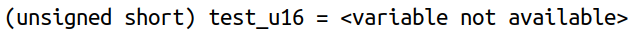
\includegraphics[width=1.0\textwidth]{lldb11.0-opt2-outofrange-edited.png}
    \label{fig:lldboutofrange}
\end{figure}

